%=============================================================================
%  Generative--Verifier Architecture for Regulation-Compliant
%  Pharmaceutical Name Generation
%  IEEE conference paper (IEEEtran, two-column).
%
%  Build:  tectonic manuscript.tex   (run twice)
%  All TikZ figures compile from this file alone. The two data figures
%  (fig_corpus, fig_strata) are regenerated by `python paper/make_figures.py`,
%  and every tabulated number is reproduced by `python paper/reproduce.py`.
%=============================================================================
\documentclass[conference]{IEEEtran}
\IEEEoverridecommandlockouts

\usepackage{cite}
\usepackage{amsmath,amssymb}
\usepackage{graphicx}
\usepackage{booktabs}
\usepackage{multirow}
\usepackage{url}
\usepackage[T1]{fontenc}
\usepackage{microtype}
\usepackage{algorithm}
\usepackage{algpseudocode}
\usepackage{tikz}
\usepackage{pgfplots}
\pgfplotsset{compat=1.18}
\usetikzlibrary{arrows.meta,positioning,fit,backgrounds,calc,shapes.geometric,decorations.pathreplacing}

\usepackage[hidelinks]{hyperref}
\graphicspath{{figures/}}

% ---- shared TikZ styles -----------------------------------------------------
\tikzset{
  blk/.style   = {draw, rounded corners=2pt, align=center, font=\scriptsize,
                  minimum height=6.5mm, inner sep=2pt, fill=black!3},
  datablk/.style = {blk, fill=black!8},
  propblk/.style = {blk, fill=blue!6},
  scrblk/.style  = {blk, fill=red!6},
  qblk/.style    = {blk, fill=green!8},
  ar/.style      = {-{Latex[length=1.6mm,width=1.2mm]}, thick},
  arf/.style     = {-{Latex[length=1.6mm,width=1.2mm]}, thick, dashed},
  lbl/.style     = {font=\scriptsize\itshape, align=center, inner sep=1pt}
}

\newcommand{\code}[1]{\texttt{\footnotesize #1}}

\begin{document}

\title{Generative--Verifier Architecture for Regulation-Compliant\\ Pharmaceutical Name Generation}

\author{%
\IEEEauthorblockN{Aviral Sharma and Vedansh Shetty}
\IEEEauthorblockA{\textit{Department of Artificial Intelligence and Data Science}\\
\textit{K.~J.~Somaiya College of Engineering, Somaiya Vidyavihar University}\\
Mumbai, India}
}

\maketitle

%=============================================================================
\begin{abstract}
Naming a medicine is a constrained search problem, not a creative one. A
nonproprietary name must carry the mandated International Nonproprietary Name
(INN) or United States Adopted Name (USAN) class stem, a proprietary name must
carry none, and both must stay orthographically and phonetically distant from
roughly twenty thousand marketed names whose confusion causes documented
dispensing errors. This paper presents a generative--verifier architecture that
couples two free-running statistical proposers to a five-check regulatory screen
and a separate, downstream quality objective, so that generation and screening
form one closed loop. The screen reimplements the algorithm family behind the
FDA Phonetic and Orthographic Computer Analysis (POCA) tool, combining
normalised Levenshtein similarity, BI-SIM bigram alignment and ALINE phonetic
alignment over a rule-based grapheme-to-phoneme converter. Against 30 documented
look-alike sound-alike pairs and 400 sampled random pairs it attains a ROC AUC of
0.997 with a mean score separation of 39.9 points. A three-seed sweep over
twenty difficulty-stratified targets screens 8,081 candidates and admits 27.8\%:
\emph{brand} targets, which carry no stem at all, accept at $0.501 \pm 0.051$
across seeds while stem-governed \emph{generic} targets accept at $0.241 \pm
0.003$, the opposite objectives the two pipelines exist to enforce. Two results
a winners-only evaluation would hide are reported: the 55--70 moderate-similarity
band absorbs 88\% of shortlisted names because a mandated stem itself forces
similarity to siblings, and the highest-weighted quality term is a near-constant
offset that does not change candidate ranking.
\end{abstract}

\begin{IEEEkeywords}
pharmaceutical nomenclature, look-alike sound-alike drug names, phonetic
similarity, constrained text generation, medication safety, regulatory
screening
\end{IEEEkeywords}

%=============================================================================
\section{Introduction}

Confusion between drug names is a persistent and measurable source of
medication error. Lambert \textit{et al.} established that orthographic and
phonetic similarity is a quantifiable risk factor for name-related dispensing
errors rather than an anecdotal one \cite{lambert1999}, and the Institute for
Safe Medication Practices maintains a standing list of name pairs implicated in
real incidents \cite{ismp}. Regulators respond to this at the point of approval:
the US Food and Drug Administration screens every proposed proprietary name with
the Phonetic and Orthographic Computer Analysis (POCA) tool \cite{fdapoca} and
publishes best-practice criteria that a sponsor is expected to have applied
before submission \cite{fdaguidance}, while the European Medicines Agency
operates an equivalent review through its (Invented) Name Review Group
\cite{emaguideline}.

The constraint set on a new name is therefore not aesthetic. A nonproprietary
name is governed by the WHO INN stem system \cite{whostem} and, in the United
States, the USAN Council \cite{usanstems}: the name must terminate in the stem
that identifies its pharmacological class, must not carry any \emph{other}
class's stem anywhere in the string, and must remain distinguishable from every
sibling that shares the same mandated ending. A proprietary name is governed by
the opposite rule. It must carry no class stem at all, since a stem in a brand
name is a false claim of class membership, and it is additionally screened for
trademark conflict and for adverse meaning in the markets where the product will
be sold.

Existing computational work addresses only one half of this problem. The
similarity-screening literature, beginning with Kondrak and Dorr's evaluation of
orthographic and phonetic measures on confusable drug names
\cite{kondrak2006,kondrak2004}, treats the candidate name as given and asks how
close it is to existing names. It does not propose names. Conversely, generative
language models can produce plausible strings but have no notion of a mandated
stem, a sibling set, or a regulatory operating point, and a model asked to
produce a beta-blocker name will happily emit a real antibiotic prefix with the
beta-blocker stem appended.

This paper describes a system that closes the loop. Its contributions are:

\begin{enumerate}
\item \textbf{A parallel pool-and-select architecture} in which two structurally
      different free proposers, a syllable grammar induced from the corpus and a
      guided character n-gram model, are both run on every request and the whole
      pool is screened before any selection is made, so a shortlist can never be
      a local optimum of whichever proposer happened to run first
      (Section~\ref{sec:orch}). Rejections return to the proposers as
      machine-readable payloads that steer the rest of the request.
\item \textbf{A five-check regulatory screen and a deliberately separate quality
      objective.} The screen reimplements the POCA family from scratch and
      extends it with INN/USAN stem conformance (including detection of foreign
      class stems embedded in otherwise compliant names), a trademark proxy,
      phonotactics and a cross-lingual lexicon. The quality objective ranks what
      survives and can never rescue a rejection, keeping the regulatory decision
      a regulatory decision (Sections~\ref{sec:verifier} and \ref{sec:quality}).
\item \textbf{An evaluation that logs every candidate ever screened}, not only
      the winners, executed over three seeds and twenty targets with brand and
      generic results reported separately. Acceptance rate, per-proposer
      contribution, the failure-code distribution and an ablation of every
      objective term are all derivable from a single committed artifact
      (Section~\ref{sec:results}).
\end{enumerate}

Two findings are negative results about the system's own design and are
presented as such: the review band regulators reserve absorbs most admissible
names in a stem-governed class, and the highest-weighted term in the quality
objective shifts every score by a near-constant amount without changing which
names are selected.

%=============================================================================
\section{Background and Related Work}

\subsection{Regulatory constraints on pharmaceutical names}

The INN system assigns a common stem to substances sharing a pharmacological
class, so that \code{-olol} identifies a beta-adrenoceptor antagonist and
\code{-prazole} a proton pump inhibitor \cite{whostem}. The stem is mandatory
and terminal for a nonproprietary name; the portion preceding it, conventionally
called the fantasy prefix, is the only part the namer controls. USAN operates a
parallel and largely harmonised list for the United States \cite{usanstems}. The
FDA's best-practice guidance for proprietary names additionally prohibits names
that overstate efficacy, imply an unapproved use, or are confusable with a
marketed product \cite{fdaguidance}, and the EMA guideline imposes comparable
conditions for centrally authorised products \cite{emaguideline}.

\subsection{Computational similarity screening}

Kondrak and Dorr evaluated a large family of string and phonetic similarity
measures against a reference set of confusable drug name pairs and reported that
combining an orthographic bigram measure, BI-SIM, with edit distance outperformed
any single measure \cite{kondrak2006,kondrak2004}. BI-SIM aligns bigram sequences
with a longest-common-subsequence recurrence in which a pair of bigrams may match
partially, recovering the transposition-style confusions that unit-cost edit
distance \cite{levenshtein1966} under-penalises. On the phonetic side, ALINE
\cite{kondrak2000} scores an optimal alignment between two phone sequences using
articulatory feature distances. Zobel and Dart established the broader point that
phonetic string matching benefits from combining orthographic and phonetic
evidence rather than choosing between them \cite{zobel1996}. Emmerton
\textit{et al.} reported an operational LASA-detection tool on similar
foundations \cite{emmerton2020}, and Lambert \textit{et al.} characterised
detection limits for identifying highly confusable names from experimental data
\cite{lambert2015}. The FDA's POCA tool implements a comparable composite and is
the practical operating reference \cite{fdapoca}.

\subsection{Generative approaches}

Constrained decoding can force a language model's output to satisfy a formal
grammar without finetuning \cite{geng2023}, and controlled sampling schemes such
as nucleus sampling govern the quality-diversity tradeoff in open-ended
generation \cite{holtzman2020}. Surveys of large language models in
pharmaceutical research and development document rapid adoption alongside a
persistent tendency to generate confident but unverifiable output
\cite{liu2024}. Neither line of work supplies what pharmaceutical naming needs,
which is not fluency but a decision procedure defensible to a regulator.

\subsection{The gap this work addresses}

Screening systems evaluate names they are given. Generative systems produce
names nobody has screened. The proposed system treats the two as one closed loop
in which the screen's structured rejections are fed back as sampling pressure
within the same request, and in which admissibility and desirability are computed
by two deliberately separate components.

%=============================================================================
\section{System Architecture}

\begin{figure*}[t]
\centering
\resizebox{\textwidth}{!}{%
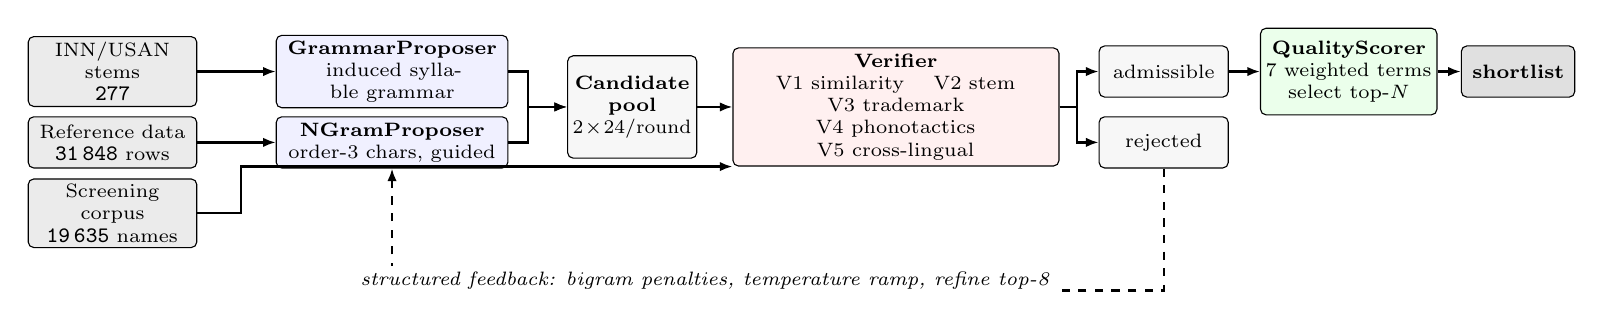
\begin{tikzpicture}[x=1cm, y=1cm]
\footnotesize
% ---------------- data column ----------------
\node[datablk, anchor=west, text width=20mm] (stem) at (0.0, 0.95)
      {INN/USAN stems\\ \code{277}};
\node[datablk, anchor=west, text width=20mm] (data) at (0.0, 0.05)
      {Reference data\\ \code{31\,848} rows};
\node[datablk, anchor=west, text width=20mm] (corp) at (0.0,-0.85)
      {Screening corpus\\ \code{19\,635} names};

% ---------------- proposers ----------------
\node[propblk, anchor=west, text width=28mm] (gram) at (3.15, 0.95)
      {\textbf{GrammarProposer}\\ induced syllable grammar};
\node[propblk, anchor=west, text width=28mm] (ngram) at (3.15, 0.05)
      {\textbf{NGramProposer}\\ order-3 chars, guided};

% ---------------- pool ----------------
\node[blk, anchor=west, text width=15mm, minimum height=13mm] (pool) at (6.85, 0.50)
      {\textbf{Candidate}\\ \textbf{pool}\\ $2\times24$/round};

% ---------------- verifier ----------------
\node[scrblk, anchor=west, text width=40mm, minimum height=15mm] (ver) at (8.95, 0.50)
      {\textbf{Verifier}\\ V1 similarity \quad V2 stem\\
       V3 trademark \quad V4 phonotactics\\ V5 cross-lingual};

% ---------------- split ----------------
\node[blk, anchor=west, text width=15mm] (adm) at (13.60, 0.95) {admissible};
\node[blk, anchor=west, text width=15mm] (rej) at (13.60, 0.05) {rejected};

% ---------------- quality and select ----------------
\node[qblk, anchor=west, text width=21mm, minimum height=11mm] (qual) at (15.65, 0.95)
      {\textbf{QualityScorer}\\ 7 weighted terms\\ select top-$N$};
\node[blk, anchor=west, text width=13mm, fill=black!12] (out) at (18.20, 0.95)
      {\textbf{shortlist}};

% ---------------- edges ----------------
\draw[ar] (stem.east) -- (gram.west);
\draw[ar] (data.east) -- ++(0.25,0) |- (ngram.west);
\draw[ar] (corp.east) -- ++(0.55,0) |- (ver.south west);
\draw[ar] (gram.east) -- ++(0.25,0) |- (pool.west);
\draw[ar] (ngram.east) -- ++(0.25,0) |- (pool.west);
\draw[ar] (pool.east) -- (ver.west);
\draw[ar] (ver.east) -- ++(0.22,0) |- (adm.west);
\draw[ar] (ver.east) -- ++(0.22,0) |- (rej.west);
\draw[ar] (adm.east) -- (qual.west);
\draw[ar] (qual.east) -- (out.west);

% feedback loop
\draw[arf] (rej.south) -- ++(0,-1.55) -| (ngram.south);
\node[lbl, fill=white, inner sep=2pt] at (8.6,-1.70)
      {structured feedback: bigram penalties, temperature ramp, refine top-8};

\end{tikzpicture}}
\caption{Request path of the proposed system. Both free proposers run in parallel
on every request and the entire pool is screened before any selection is made,
so a shortlist can never be a local optimum of whichever proposer ran first.
Rejections return to the statistical proposer as machine-readable payloads,
never as prose.}
\label{fig:arch}
\end{figure*}

\subsection{Reference data and corpus construction}

The data layer assembles a screening universe from primary regulatory sources:
the openFDA National Drug Code directory \cite{openfda}, the RxNorm ingredient
and brand-name vocabularies \cite{rxnorm}, and the EMA medicines register, plus
a curated INN/USAN stem table of 277 entries. It is live-first with a committed
static snapshot as fallback, and every run records which path executed, because
degrading silently to a smaller universe would inflate every distinctiveness
margin reported.

The raw feed is not usable as a name corpus. The NDC directory mixes true drug
names with over-the-counter product descriptions, so a filter admits only single
alphabetic tokens of 4 to 25 characters that are not dosage forms, salts or
counter-ions, or marketing modifiers. Multi-ingredient generic entries are split
on whitespace rather than discarded, because each component of a combination
product is itself a real active-ingredient name. Table~\ref{tab:corpus} and
Fig.~\ref{fig:corpus} report the result; the surviving names have a mean length
of 9.7 characters and 4.0 syllables for generics against 7.8 and 3.1 for brands,
and these empirical distributions are the reference used by the shape term of the
objective.

\begin{table}[t]
\caption{Corpus composition of the reported run.}
\label{tab:corpus}
\centering
\footnotesize
\setlength{\tabcolsep}{3.5pt}
\begin{tabular}{lrl}
\toprule
Quantity & Value & Note \\
\midrule
Raw snapshot rows            & 31\,848 & multi-source union \\
Screening universe (unique)  & 19\,635 & what the verifier measures from \\
\quad generic names          & 12\,542 & \\
\quad brand names            &  9\,397 & trademark screen pool: 9\,402 \\
Noise tokens filtered        & 48\,799 & dosage forms, salts, marketing \\
Fantasy prefixes extracted   &  1\,700 & 1\,608 unique; n-gram training set \\
Stem matches in corpus       &  1\,817 & 14.5\% of generic tokens \\
Brand marks (training)       &  4\,672 & \\
Blocklisted morphemes        &  1\,212 & class-signalling fragments \\
INN/USAN stems               &     277 & suffix and embedded matching \\
\bottomrule
\end{tabular}
\end{table}

\begin{figure*}[t]
\centering
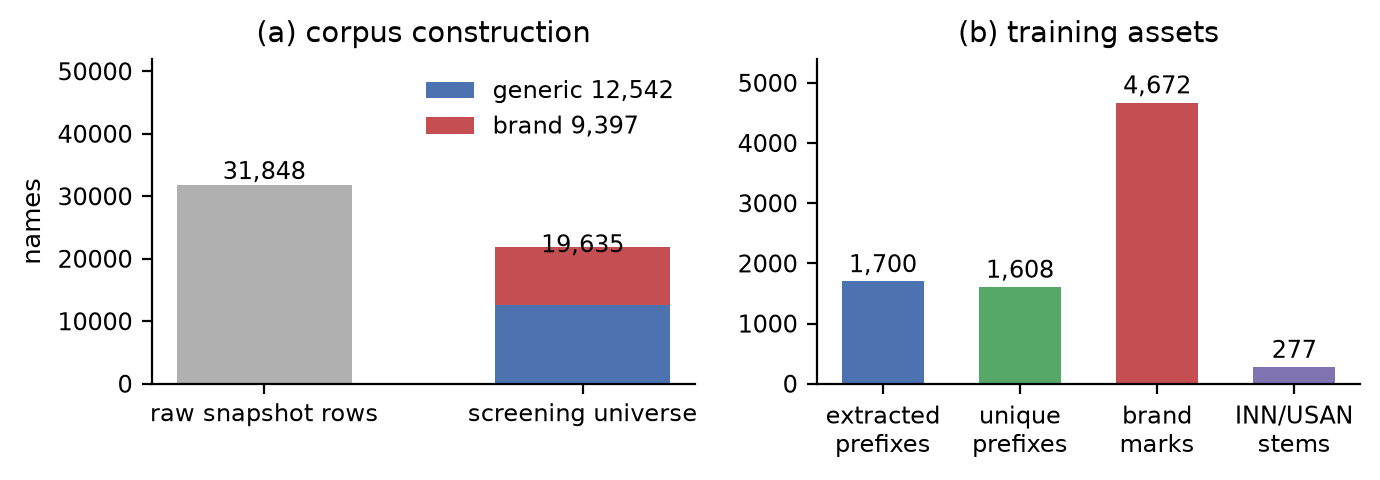
\includegraphics[width=\textwidth]{fig_corpus.png}
\caption{Corpus statistics drawn by \code{paper/make\_figures.py} from the
committed manifest. (a) Of 31\,848 raw snapshot rows, filtering admits a
19\,635-name screening universe split 12\,542 generic / 9\,397 brand. (b) The
training corpora the two proposers are fit on: 1\,608 unique fantasy prefixes, a
4\,672-mark brand set, and the 277-row INN/USAN stem table.}
\label{fig:corpus}
\end{figure*}

\subsection{Proposers}

\subsubsection{Induced syllable grammar}
The grammar proposer samples a fantasy prefix from a syllable inventory
\emph{induced} from the corpus rather than hand-specified. Real prefixes are
parsed into onset, nucleus and coda units, and new syllables are drawn from the
empirical positional frequencies (Fig.~\ref{fig:grammar}). Induction over the
1\,700 extracted prefixes yields 39 attested onsets for the generic register and
56 for the brand register, with an empirical syllable-count distribution of
$\{1{:}233,\, 2{:}846,\, 3{:}517,\, 4{:}99,\, 5{:}4\}$.

The design consequence is structural rather than statistical. Because
recombination happens at the syllable level, the proposer cannot reproduce a
whole morpheme such as \code{erythro} unless \code{e}, \code{ry} and \code{thro}
are independently resampled in order, so the memorisation failure mode is
excluded by the representation rather than penalised after the fact. When the
mandated stem begins with a vowel the sampler is further constrained to emit a
consonant-final prefix, avoiding a vowel pile-up at the join.

\begin{figure}[t]
\centering
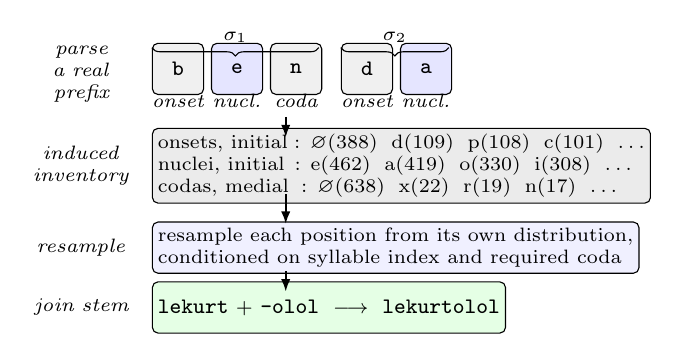
\begin{tikzpicture}[x=1cm, y=1cm]
\footnotesize
% ---- row labels ----
\node[lbl, anchor=east, text width=13mm] at (1.30, 1.78) {parse a real\\ prefix};
\node[lbl, anchor=east, text width=13mm] at (1.30, 0.62) {induced\\ inventory};
\node[lbl, anchor=east, text width=13mm] at (1.30,-0.42) {resample};
\node[lbl, anchor=east, text width=13mm] at (1.30,-1.18) {join stem};

% ---- row 1: the real prefix "benda" split into units ----
\node[blk, anchor=west, minimum width=6.5mm, fill=black!6] (u1) at (1.50,1.85) {\code{b}};
\node[blk, anchor=west, minimum width=6.5mm, fill=blue!10] (u2) at (2.25,1.85) {\code{e}};
\node[blk, anchor=west, minimum width=6.5mm, fill=black!6] (u3) at (3.00,1.85) {\code{n}};
\node[blk, anchor=west, minimum width=6.5mm, fill=black!6] (u4) at (3.90,1.85) {\code{d}};
\node[blk, anchor=west, minimum width=6.5mm, fill=blue!10] (u5) at (4.65,1.85) {\code{a}};
\node[lbl] at (1.83,1.44) {onset};
\node[lbl] at (2.58,1.44) {nucl.};
\node[lbl] at (3.33,1.44) {coda};
\node[lbl] at (4.23,1.44) {onset};
\node[lbl] at (4.98,1.44) {nucl.};
\draw[decorate, decoration={brace, amplitude=3pt}] (3.62,2.12) -- (1.50,2.12)
  node[midway, above, font=\scriptsize, inner sep=1.5pt] {$\sigma_1$};
\draw[decorate, decoration={brace, amplitude=3pt}] (5.27,2.12) -- (3.90,2.12)
  node[midway, above, font=\scriptsize, inner sep=1.5pt] {$\sigma_2$};

% ---- row 2: induced inventory ----
\node[datablk, anchor=west, align=left] (inv) at (1.50,0.62)
  {onsets, initial\;: $\varnothing$(388)\; d(109)\; p(108)\; c(101)\; $\ldots$\\
   nuclei, initial\;\,: e(462)\; a(419)\; o(330)\; i(308)\; $\ldots$\\
   codas, medial\;\;: $\varnothing$(638)\; x(22)\; r(19)\; n(17)\; $\ldots$};

% ---- row 3: resampling ----
\node[propblk, anchor=west, align=left] (samp) at (1.50,-0.42)
  {resample each position from its own distribution,\\
   conditioned on syllable index and required coda};

% ---- row 4: output ----
\node[blk, anchor=west, fill=green!10] (outn) at (1.50,-1.18)
  {\code{lekurt} $+$ \code{-olol} $\;\longrightarrow\;$ \code{lekurtolol}};

% ---- arrows down the spine ----
\draw[ar] (3.20,1.24) -- (3.20,0.98);
\draw[ar] (3.20,0.26) -- (3.20,-0.12);
\draw[ar] (3.20,-0.72) -- (3.20,-0.98);
\end{tikzpicture}
\caption{Syllable-grammar induction on the real corpus prefix \code{benda}.
Counts are observed positional frequencies over the 1\,700 extracted prefixes;
$\varnothing$ is an empty onset or coda. Onsets are maximised, so an
intervocalic consonant becomes a coda only when the remainder is not an attested
word-initial onset.}
\label{fig:grammar}
\end{figure}

\subsubsection{Guided character n-gram model}
The statistical proposer is an order-3 character model with add-$k$ smoothing
trained on the same prefix set. Guidance operates across a batch rather than
within a draw (Fig.~\ref{fig:ngram}). Bigrams appearing in the colliding region
of a rejected candidate are down-weighted but never zeroed, so the search space
stays connected, and the sampling temperature rises with the number of
consecutive failed rounds. Each output slot is drawn three times and the draw
with the highest verifier-free reward is kept, which approximates optimising for
quality during proposal at microsecond rather than millisecond cost.

\begin{figure}[t]
\centering
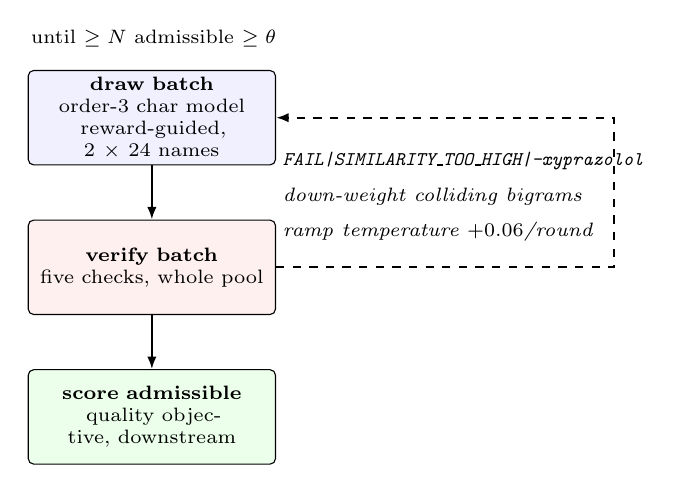
\begin{tikzpicture}[x=1cm, y=1cm]
\footnotesize
\node[propblk, anchor=west, text width=30mm, minimum height=12mm] (draw) at (0.70, 1.90)
      {\textbf{draw batch}\\ order-3 char model\\
       reward-guided, $2\times24$ names};
\node[scrblk, anchor=west, text width=30mm, minimum height=12mm] (verify) at (0.70, 0.00)
      {\textbf{verify batch}\\ five checks, whole pool};
\node[qblk, anchor=west, text width=30mm, minimum height=12mm] (score) at (0.70,-1.90)
      {\textbf{score admissible}\\ quality objective, downstream};

\draw[ar] (draw.south) -- (verify.north);
\draw[ar] (verify.south) -- (score.north);

\draw[arf] (verify.east) -- (8.15, 0.00) |- (draw.east);
\node[lbl, font=\scriptsize] at (2.30, 2.90) {until $\ge N$ admissible $\ge \theta$};

\node[lbl, anchor=west] at (3.90, 1.35)
      {\code{\scriptsize FAIL|SIMILARITY\_TOO\_HIGH|-xyprazolol}};
\node[lbl, anchor=west] at (3.90, 0.90) {down-weight colliding bigrams};
\node[lbl, anchor=west] at (3.90, 0.45) {ramp temperature $+0.06$/round};
\end{tikzpicture}
\caption{Guided n-gram proposal loop. Bigrams from rejection payloads steer
later draws in the same request; admissible names alone proceed to the quality
objective. Everything that fails a check is logged, never silently dropped.}
\label{fig:ngram}
\end{figure}

\subsection{The screening component}
\label{sec:verifier}

The verifier answers one question, whether a name \emph{may} exist, through five
checks. It is a from-scratch implementation with no model downloads and no
network calls on the default path, which is what makes a results run
byte-reproducible.

\paragraph{V1, similarity}
For candidate $a$ and corpus name $b$, orthographic similarity combines
normalised Levenshtein similarity $L$ with BI-SIM $B$, and the composite blends
that with ALINE phonetic similarity $P$ computed over rule-based phoneme
transcriptions:
\begin{align}
L(a,b) &= 1 - \frac{d_{\mathrm{lev}}(a,b)}{\max(|a|,|b|)}, \\
O(a,b) &= w_{L}\,L(a,b) + w_{B}\,B(a,b), \\
S(a,b) &= 100 \cdot \big[\, w_{O}\,O(a,b) + w_{P}\,P(a,b) \,\big],
\end{align}
with $w_L = w_B = w_O = w_P = 0.5$, reproducing the equal-weight configuration
of the published POCA behaviour. The composite risk score of a candidate is
$\max_b S(a,b)$ over the screening universe, computed after a bigram prefilter
that reduces the phonetic comparison to a pool of 150 nearest candidates.

Two operating points partition the score, following the published reading of
POCA output: $S \geq 70$ is a hard rejection, $55 \leq S < 70$ is a
moderate-similarity band admissible with review, and $S < 55$ is low risk
(Fig.~\ref{fig:bands}). When the target class mandates a stem, the stem is
stripped from both strings before scoring siblings that share it, so that
distinctiveness measures the part the namer actually controls rather than
penalising a name for complying with the regulation that forced the ending on
it. Sibling comparison uses a separate and stricter cutoff of 75.

\paragraph{V2, stem conformance}
For a generic target the terminal stem must match the requested class, at least
two characters of fantasy prefix must precede it, and no \emph{foreign} class
stem may appear embedded elsewhere in the string. The last condition is not
redundant. Names such as \code{cillinolol} carry a correct terminal stem and a
contradictory internal one, and the INN system treats a misleading internal stem
the same way it treats a misleading terminal one. For a brand target the
condition inverts: any stem in stem position is a false class claim and fails.

\paragraph{V3, trademark collision}
The candidate is scored against the 9\,402 marketed proprietary names using the
same composite, with a rejection at 70. This is explicitly a proxy for
marketed-name collision, not a registered trademark class search.

\paragraph{V4, phonotactic well-formedness}
The name is transcribed by a rule-based grapheme-to-phoneme converter,
syllabified by sonority, and scored as $0.6\,\phi + 0.4\,\tau$ where $\phi$ is
phonotactic legality (cluster admissibility, consonant and vowel run limits) and
$\tau$ is corpus typicality under a character trigram model of the appropriate
register. A name yielding no vowel nucleus is rejected outright; the floor is
0.45.

\paragraph{V5, cross-lingual and implied claim}
A curated lexicon of 68 adverse terms across eight major markets (Spanish,
French, German, Italian, Portuguese, Japanese, Chinese, Hindi) is matched as
substring and by ALINE similarity at a 0.88 cutoff, and 25 efficacy-implying
fragments are flagged as warnings. This is a lexicon lookup, not a phonological
model.

\begin{figure}[t]
\centering
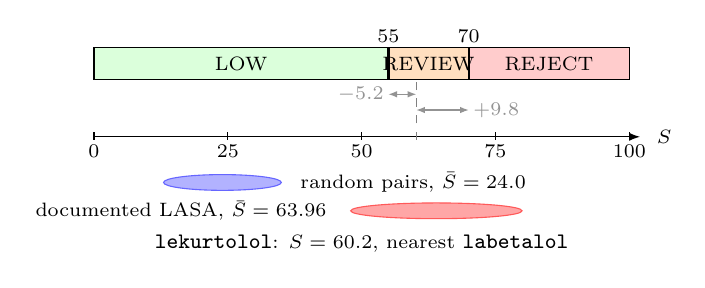
\begin{tikzpicture}[x=0.068cm, y=1cm]
\footnotesize
% ---- band strip ----
\fill[green!14] (0,1.05) rectangle (55,1.45);
\fill[orange!25] (55,1.05) rectangle (70,1.45);
\fill[red!20]   (70,1.05) rectangle (100,1.45);
\draw (0,1.05) rectangle (100,1.45);
\draw[thick] (55,1.05) -- (55,1.45);
\draw[thick] (70,1.05) -- (70,1.45);
\node[font=\scriptsize] at (27.5,1.25) {LOW};
\node[font=\scriptsize] at (62.5,1.25) {REVIEW};
\node[font=\scriptsize] at (85,1.25) {REJECT};
\node[font=\scriptsize, anchor=south, inner sep=1pt] at (55,1.47) {55};
\node[font=\scriptsize, anchor=south, inner sep=1pt] at (70,1.47) {70};

% ---- margins of the worked candidate ----
\draw[{Latex[length=1.1mm]}-{Latex[length=1.1mm]}, gray!85] (55,0.86) -- (60.21,0.86);
\node[font=\scriptsize, anchor=east, inner sep=1.5pt, text=gray!85] at (55,0.86) {$-5.2$};
\draw[{Latex[length=1.1mm]}-{Latex[length=1.1mm]}, gray!85] (60.21,0.66) -- (70,0.66);
\node[font=\scriptsize, anchor=west, inner sep=1.5pt, text=gray!85] at (70,0.66) {$+9.8$};

% ---- axis ----
\draw[-{Latex[length=1.4mm]}] (0,0.32) -- (102,0.32);
\foreach \x in {0,25,50,75,100}
  \draw (\x,0.38) -- (\x,0.28) node[below, font=\scriptsize, inner sep=1.5pt] {\x};
\node[font=\scriptsize, anchor=west, inner sep=2pt] at (104,0.32) {$S$};

% ---- measured distributions ----
\draw[fill=blue!30, draw=blue!60] (24.0,-0.26) ellipse (11 and 0.10);
\node[font=\scriptsize, anchor=west] at (37,-0.26) {random pairs, $\bar{S}=24.0$};
\draw[fill=red!35, draw=red!65] (63.96,-0.62) ellipse (16 and 0.10);
\node[font=\scriptsize, anchor=east] at (45,-0.62) {documented LASA, $\bar{S}=63.96$};

% ---- worked candidate ----
\draw[dashed, gray] (60.21,0.28) -- (60.21,1.05);
\node[font=\scriptsize, anchor=north] at (50,-0.82)
  {\code{lekurtolol}: $S=60.2$, nearest \code{labetalol}};
\end{tikzpicture}
\caption{The two-cutoff decision structure, drawn to scale, with the measured
mean composite scores of the 400 random and 30 documented look-alike sound-alike
pairs superimposed. A candidate reports \emph{two} margins. Reporting only the
margin to 70, as an earlier version did, makes a name inside the review band
read as comfortable.}
\label{fig:bands}
\end{figure}

\subsection{The quality objective}
\label{sec:quality}

The verifier decides admissibility; it says nothing about whether a name is any
good. That distinction matters because an earlier version of this system,
measuring risk alone, accepted \code{erythroolol}, \code{amoxiolol} and
\code{acycloolol}: three real drug prefixes with a beta-blocker stem appended,
which is exactly the cross-class misidentification the stem system exists to
prevent.

A separate scorer therefore computes seven weighted terms in $[0,1]$, with two
profiles because the objectives genuinely differ (Table~\ref{tab:weights}). Two
choices are worth stating. \emph{Distinctiveness} scores headroom below the
review line at 55, not the reject line at 70, so a grey-band name scores poorly
rather than comfortably. \emph{Typicality} is scored as a band targeting 0.40 to
0.70 rather than a maximum, because maximising corpus likelihood is precisely
the objective that produces memorised prefixes.

Critically, the scorer is never consulted by the admissibility decision. It ranks
what survives and cannot rescue a rejection, which is what keeps the regulatory
claim a regulatory claim rather than a preference model.

\begin{table}[t]
\caption{Quality objective. Weights sum to 1.0 within each profile;
a dash marks a term that does not exist for that profile.}
\label{tab:weights}
\centering
\footnotesize
\setlength{\tabcolsep}{3.5pt}
\begin{tabular}{lccl}
\toprule
Term & Gen. & Brand & Measures \\
\midrule
distinctiveness  & 0.24 & 0.24 & headroom below the review line \\
novelty          & 0.20 & 0.14 & verbatim reuse of a real fragment \\
morpheme hygiene & 0.16 & --   & carrying another class's stem \\
stem avoidance   & --   & 0.16 & any stem is a false class claim \\
memorability     & --   & 0.15 & short, few syllables, clean CV \\
pronounceability & 0.14 & 0.14 & phonotactic legality, ease \\
shape            & 0.10 & --   & length, syllables vs.\ real names \\
seam             & 0.09 & 0.09 & hygiene at the prefix/stem join \\
typicality       & 0.07 & 0.08 & plausible without being derivative \\
\bottomrule
\end{tabular}
\end{table}

\subsection{Pool-and-select orchestration}
\label{sec:orch}

Algorithm~\ref{alg:pipeline} states the request path. Nothing is discarded
before it has been screened. An early-exit cascade optimises for cost: if the
first proposer clears the bar with a margin of 1.04 it stops, and never learns
that the other had a margin of 15 on the same call. Pooling screens everything
before choosing, so selection cannot be a local optimum of proposer ordering.
Sampling stops only when at least $N$ admissible candidates clear a configured
quality target $\theta$; there is no separate escalation stage to skip.

Rejections drive two mechanisms. Bigrams drawn from the machine-readable payload
of each rejection signal, specifically the colliding name, the offending sibling
and the foreign morpheme, become sampling penalties for the rest of the request.
Separately, the eight highest-quality rejects are sent through up to three
targeted edit rounds, because editing a candidate that scored 61 and missed on
one code is the cheapest quality in the system, while editing one that scored 20
is wasted work.

\begin{algorithm}[t]
\caption{Generative--verifier pool-and-select generation}
\label{alg:pipeline}
\begin{algorithmic}[1]
\footnotesize
\Require target type $t$, class $c$, stem $s$, shortlist size $N$, seed
\State $\mathcal{E} \gets \emptyset$;\; $\mathcal{A} \gets \emptyset$
       \Comment{all screened; admissible}
\For{round $r = 1 \ldots R_{\max}$}
  \State $\mathcal{P} \gets \bigcup_{p \in \{\text{grammar},\text{ngram}\}} p.\textsc{Propose}(24, \text{ctx})$
  \ForAll{$n \in \mathcal{P} \setminus \textsc{Seen}$}
    \State $\rho \gets \textsc{Verify}(n, t, c, s)$;\; $q \gets \textsc{Quality}(n, \rho, t, s)$
    \State $\mathcal{E} \gets \mathcal{E} \cup \{(n,\rho,q)\}$
    \If{$\rho.\textit{pass}$} $\mathcal{A} \gets \mathcal{A} \cup \{(n,\rho,q)\}$
    \Else{} \textsc{LearnFromRejection}(ctx, $n$, $\rho$) \EndIf
  \EndFor
  \ForAll{$n \in \textsc{TopK}(\mathcal{P} \setminus \mathcal{A}, 8)$ by $q$}
    \State refine $n$ for up to 3 rounds; screen and score each edit
  \EndFor
  \If{$|\{a \in \mathcal{A} : q_a \geq \theta\}| \geq N$} \textbf{break} \EndIf
\EndFor
\State \Return top-$N$ of $\mathcal{A}$ by quality, and $\mathcal{E}$ as the audit log
\end{algorithmic}
\end{algorithm}

%=============================================================================
\section{Experimental Setup}
\label{sec:setup}

The open-source implementation \code{pharma\_name\_gen} is built by a single
builder used by the notebook, the web application and the sweep harness, so no
entry point can silently run a different configuration. All numbers below are
reproduced offline from the committed data snapshot (fingerprint
\code{d9cc79de5be14f36}), by \code{paper/reproduce.py}, with no network access and
no API keys. The reported figures are not configuration-specific artefacts:
executed against \emph{live} openFDA and RxNorm feeds, the discrimination
experiment returns the identical corpus fingerprint and identical statistics on
the same 30 positive and 400 negative pairs.

The pipeline configuration is 24 candidates per proposer per round, at most 4
rounds, shortlist size 10, up to 3 refinement rounds over the top 8 rejects,
temperature 1.0 with a ramp of 0.06 per failed round, 3 reward-guided draws per
slot, and a quality target $\theta = 62.0$. The verifier configuration is the
threshold set given in Section~\ref{sec:verifier} with stem-aware similarity
enabled, top-$k$ of 5, a prefilter pool of 600 and a phonetic pool of 150.

Reproducibility is enforced structurally. Trained artefacts are
content-addressed on the corpus fingerprint plus a configuration hash, so
changing the stem table produces a different key and a stale model is simply not
found. Every run emits a manifest recording the fingerprint, data mode, source
record counts, thresholds, weights and git commit. A suite of 35 tests,
including an assertion that seeded runs are byte-identical, passes offline.

The sweep spans twenty targets chosen to cover the difficulty range rather than
sampled at random, since a sweep over easy classes only would report a
flattering acceptance rate that says nothing. Classes are stratified as
\emph{roomy} (few siblings, short names viable), \emph{crowded} (many siblings,
high intra-stem pressure), \emph{saturated} (dozens of recent entrants, long
stems), and \emph{brand} (no stem, inverted objective). Because the brand
register is the opposite objective rather than an easier generic class, the
brand cell set was widened from two to six therapeutic contexts
(cardiovascular, oncology, CNS/neurology, anti-infective, respiratory,
dermatology) so that the brand/generic comparison rests on six cells, not two.
The whole sweep is run at three seeds, $\{1,2,3\}$, so the headline rates are
reported as mean $\pm$ standard deviation across seeds rather than as a single
point estimate; a full sweep screens roughly 2\,700 candidates and runs in about
twenty minutes on a consumer CPU.

%=============================================================================
\section{Results}
\label{sec:results}

\subsection{Does the screen discriminate?}

The screening component is validated independently of anything the generator
produces. Positives are 30 pairs from the FDA Name Differentiation Project and
the ISMP list of confused drug names \cite{ismp}, a far stronger label than
visual resemblance because each pair has caused documented dispensing errors.
Negatives are 400 pairs sampled uniformly from the screening corpus
(Table~\ref{tab:disc}, Figs.~\ref{fig:hist} and \ref{fig:roc}).

\begin{table}[t]
\caption{Discrimination of the composite similarity score.}
\label{tab:disc}
\centering
\footnotesize
\begin{tabular}{lr}
\toprule
Quantity & Value \\
\midrule
Documented confusable pairs, $n$ & 30 \\
Random corpus pairs, $n$ & 400 \\
Mean composite, confusable & 63.96 \\
Mean composite, random & 24.04 \\
Separation & 39.91 \\
ROC AUC & 0.9970 \\
\midrule
Sensitivity / specificity at 55 (review) & 0.767 / 1.000 \\
Sensitivity / specificity at 70 (reject) & 0.367 / 1.000 \\
Youden-optimal threshold ($J = 0.952$) & 40.0 \\
Sensitivity / specificity at 40 & 0.967 / 0.985 \\
\bottomrule
\end{tabular}
\end{table}

\begin{figure}[t]
\centering
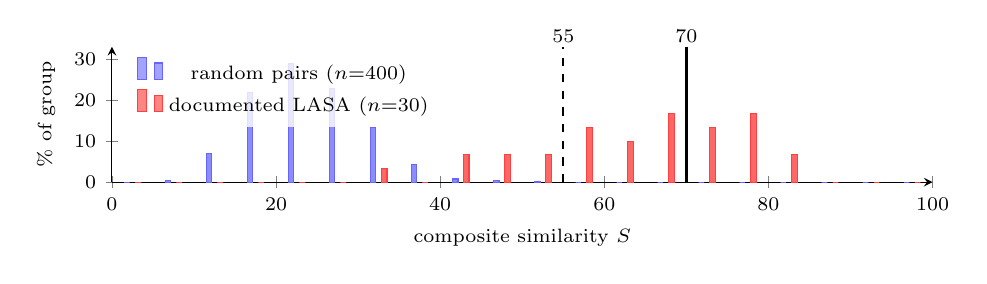
\begin{tikzpicture}
\begin{axis}[
  width=0.99\columnwidth, height=3.3cm,
  ybar, bar width=2.0pt,
  xlabel={composite similarity $S$}, ylabel={\% of group},
  xmin=0, xmax=100, ymin=0, ymax=33,
  xtick={0,20,40,60,80,100},
  label style={font=\scriptsize}, tick label style={font=\scriptsize},
  legend style={font=\scriptsize, at={(0.02,0.97)}, anchor=north west,
                draw=none, fill=white, fill opacity=0.8, text opacity=1},
  axis lines=left, enlarge x limits=false, clip=false
]
\addplot[fill=blue!45, draw=blue!60] coordinates {
(2.5,0)(7.5,0.50)(12.5,7.00)(17.5,21.75)(22.5,29.00)(27.5,22.75)(32.5,13.25)
(37.5,4.25)(42.5,0.75)(47.5,0.50)(52.5,0.25)(57.5,0)(62.5,0)(67.5,0)(72.5,0)
(77.5,0)(82.5,0)(87.5,0)(92.5,0)(97.5,0)};
\addlegendentry{random pairs ($n{=}400$)}
\addplot[fill=red!60, draw=red!75] coordinates {
(2.5,0)(7.5,0)(12.5,0)(17.5,0)(22.5,0)(27.5,0)(32.5,3.33)(37.5,0)
(42.5,6.67)(47.5,6.67)(52.5,6.67)(57.5,13.33)(62.5,10.00)(67.5,16.67)
(72.5,13.33)(77.5,16.67)(82.5,6.67)(87.5,0)(92.5,0)(97.5,0)};
\addlegendentry{documented LASA ($n{=}30$)}
\draw[dashed, thick, black] (axis cs:55,0) -- (axis cs:55,33)
  node[above, font=\scriptsize, inner sep=1pt] {55};
\draw[thick, black] (axis cs:70,0) -- (axis cs:70,33)
  node[above, font=\scriptsize, inner sep=1pt] {70};
\end{axis}
\end{tikzpicture}
\caption{Score distributions for documented confusable pairs and random corpus
pairs, binned at width 5 and normalised within each group so that the two very
different sample sizes are comparable. The distributions are almost disjoint,
which is what a ROC AUC of 0.997 means concretely, and the residual overlap
sits entirely below the review line.}
\label{fig:hist}
\end{figure}

\begin{figure}[t]
\centering
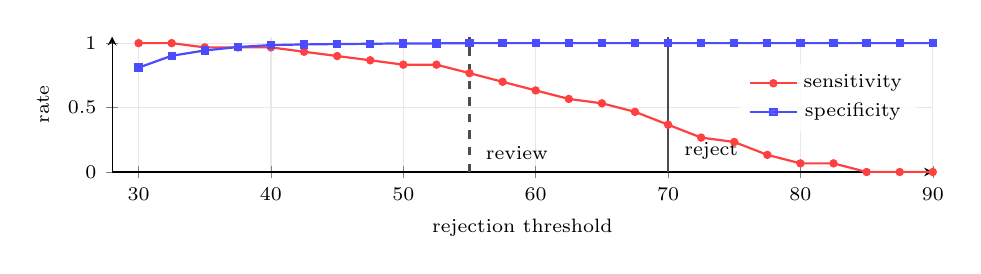
\begin{tikzpicture}
\begin{axis}[
  width=0.99\columnwidth, height=3.3cm,
  xlabel={rejection threshold}, ylabel={rate},
  xmin=28, xmax=90, ymin=0, ymax=1.05,
  xtick={30,40,50,60,70,80,90},
  label style={font=\scriptsize}, tick label style={font=\scriptsize},
  legend style={font=\scriptsize, at={(0.98,0.55)}, anchor=east,
                draw=none, fill=white, fill opacity=0.8, text opacity=1},
  axis lines=left, grid=major, grid style={gray!18}
]
\addplot[red!75, mark=*, mark size=1.1pt, thick] coordinates {
(30,1.000)(32.5,1.000)(35,0.967)(37.5,0.967)(40,0.967)(42.5,0.933)(45,0.900)
(47.5,0.867)(50,0.833)(52.5,0.833)(55,0.767)(57.5,0.700)(60,0.633)(62.5,0.567)
(65,0.533)(67.5,0.467)(70,0.367)(72.5,0.267)(75,0.233)(77.5,0.133)(80,0.067)
(82.5,0.067)(85,0.000)(87.5,0.000)(90,0.000)};
\addlegendentry{sensitivity}
\addplot[blue!70, mark=square*, mark size=1.1pt, thick] coordinates {
(30,0.810)(32.5,0.902)(35,0.943)(37.5,0.970)(40,0.985)(42.5,0.990)(45,0.993)
(47.5,0.995)(50,0.998)(52.5,0.998)(55,1.000)(57.5,1.000)(60,1.000)(62.5,1.000)
(65,1.000)(67.5,1.000)(70,1.000)(72.5,1.000)(75,1.000)(77.5,1.000)(80,1.000)
(82.5,1.000)(85,1.000)(87.5,1.000)(90,1.000)};
\addlegendentry{specificity}
\draw[dashed, thick, black!70] (axis cs:55,0) -- (axis cs:55,1.05);
\draw[thick, black!70] (axis cs:70,0) -- (axis cs:70,1.05);
\node[font=\scriptsize, anchor=south west] at (axis cs:55.5,0.02) {review};
\node[font=\scriptsize, anchor=south west] at (axis cs:70.5,0.02) {reject};
\end{axis}
\end{tikzpicture}
\caption{Operating characteristics. Specificity against random pairs is already
1.000 at the review line of 55, so raising the cutoff to 70 buys no additional
specificity and costs 0.40 in sensitivity. This is the direct quantitative
argument for treating 55--70 as a reportable band rather than passing it
silently.}
\label{fig:roc}
\end{figure}

The finding worth stating is not the AUC but the shape of Fig.~\ref{fig:roc}:
specificity saturates at 1.000 by the review line, so every threshold point
above 55 is paid for purely in sensitivity. At the reject cutoff of 70 the
screen recovers only 11 of the 30 documented confusable pairs. A system
reporting a binary pass at 70 would silently discard most of its own detection
capability; the two-cutoff design is what preserves it.

\subsection{Which similarity measure carries the discrimination?}

Each weight was zeroed in turn and the AUC recomputed against 300 sampled
negatives (Table~\ref{tab:ablate-sim}). The orthographic component is
load-bearing; removing the phonetic and BI-SIM terms changes the AUC by less
than 0.001. The methodology must reflect this: the claim that phonetic alignment
contributes is not supported at this operating point by these 30 pairs, though
it is retained because the pairs it targets, homophones with divergent
spellings, are under-represented in a set of 30.

\begin{table}[t]
\caption{Similarity-component ablation. One weight zeroed at a time,
30 positive and 300 negative pairs.}
\label{tab:ablate-sim}
\centering
\footnotesize
\begin{tabular}{lccr}
\toprule
Component zeroed & Weight & ROC AUC & $\Delta$ \\
\midrule
(none removed)              & --   & 0.9974 & \phantom{$-$}0.0000 \\
$w_{\mathrm{orthographic}}$ & 0.5  & 0.9892 & $-$0.0082 \\
$w_{\mathrm{levenshtein}}$  & 0.5  & 0.9963 & $-$0.0011 \\
$w_{\mathrm{phonetic}}$     & 0.5  & 0.9969 & $-$0.0005 \\
$w_{\mathrm{bi\text{-}sim}}$& 0.5  & 0.9974 & \phantom{$-$}0.0001 \\
\bottomrule
\end{tabular}
\end{table}

\subsection{Does pool-and-select beat independent strategies?}

The predecessor architecture exposed four peer generation strategies, each
running its own end-to-end loop and producing the whole shortlist alone. Its
verbatim output on the \code{-olol} class is scored here by the \emph{same}
quality function against the \emph{same} corpus, which is the only way to turn
the comparison into a number rather than an assertion, since the earlier system
had no quality function at all. Table~\ref{tab:arch} and Fig.~\ref{fig:archfig}
report the comparison.

\begin{table}[t]
\caption{Architecture comparison on \textnormal{\texttt{-olol}}, same corpus, same screen,
same seed. Per-component figures are means over each architecture's output.}
\label{tab:arch}
\centering
\footnotesize
\begin{tabular}{lcc}
\toprule
 & v1: four strategies & v2: pool-and-select \\
\midrule
Candidates returned      & 15   & 10   \\
Mean quality             & 55.38 & \textbf{67.33} \\
Best quality             & 72.63 & 68.98 \\
Mean composite risk      & 59.31 & 59.09 \\
Low-band names           & 4     & 1    \\
\midrule
\multicolumn{3}{l}{\textit{Mean per-component quality}} \\
\quad novelty            & 0.560 & \textbf{0.928} \\
\quad seam               & 0.737 & \textbf{1.000} \\
\quad morpheme hygiene   & 0.879 & \textbf{1.000} \\
\quad pronounceability   & 0.936 & \textbf{0.979} \\
\quad shape              & 0.819 & \textbf{0.921} \\
\quad typicality         & 0.179 & 0.118 \\
\quad distinctiveness    & 0.040 & 0.001 \\
\bottomrule
\end{tabular}
\end{table}

\begin{figure}[t]
\centering
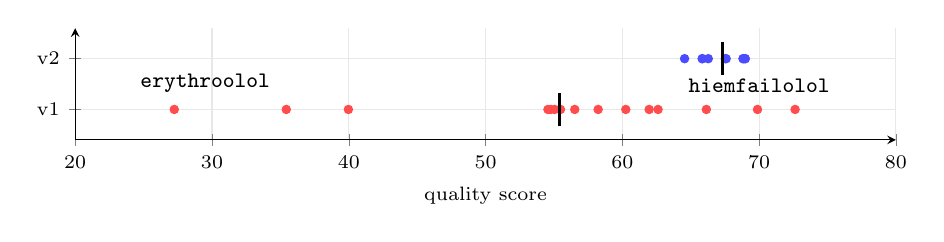
\begin{tikzpicture}
\begin{axis}[
  width=0.99\columnwidth, height=3.0cm,
  xlabel={quality score}, xmin=20, xmax=80,
  ytick={1,2}, yticklabels={v1, v2},
  ymin=0.4, ymax=2.6,
  label style={font=\scriptsize}, tick label style={font=\scriptsize},
  axis lines=left, grid=major, grid style={gray!18},
  clip=false
]
\addplot[only marks, mark=*, mark size=1.5pt, red!70] coordinates {
(27.24,1)(35.43,1)(39.97,1)(54.56,1)(54.77,1)(55.05,1)(55.48,1)(56.52,1)
(58.23,1)(60.25,1)(61.96,1)(62.61,1)(66.14,1)(69.88,1)(72.63,1)};
\addplot[only marks, mark=*, mark size=1.5pt, blue!70] coordinates {
(64.55,2)(65.84,2)(65.85,2)(66.28,2)(67.53,2)(67.59,2)(68.83,2)(68.83,2)
(68.98,2)(68.98,2)};
\addplot[only marks, mark=|, mark size=6pt, black, very thick] coordinates {
(55.38,1)(67.33,2)};
\node[font=\scriptsize, anchor=south] at (axis cs:29.5,1.14) {\code{erythroolol}};
\node[font=\scriptsize, anchor=south] at (axis cs:70.0,1.14) {\code{hiemfailolol}};
\end{axis}
\end{tikzpicture}
\caption{Per-candidate quality for the two architectures on the same class,
corpus and seed; vertical bars mark the means. The predecessor's spread is the
point: one candidate above every v2 name and three below 40.}
\label{fig:archfig}
\end{figure}

Two details in Fig.~\ref{fig:archfig} matter more than the mean. The
predecessor's best name, \code{hiemfailolol}, outscores every pool-and-select
candidate, so the improvement is not a higher ceiling but a higher floor: v2's
worst candidate scores 64.55 against a v1 minimum of 27.24, and the variance
collapses. The three worst v1 names, \code{erythroolol}, \code{vancicloolol} and
\code{acycloolol}, are all real drug prefixes with a beta-blocker stem appended,
the failure mode the induced grammar structurally excludes and the
morpheme-hygiene term penalises; that term rises from 0.879 to 1.000.

Reproducibility was verified directly: three independent invocations with the
same seed returned byte-identical shortlists.

\subsection{Brand versus generic across three seeds}
\label{sec:res:sweep}

The sweep logs one row per candidate ever screened, accepted or not. Across
twenty targets and three seeds it screened 8\,081 candidates and admitted
2\,247 of them ($27.8\%$); each seed screened roughly 2\,700 candidates and
each returned a full shortlist of 10 for every target, entirely on CPU.

The comparison the two pipelines exist to make is reported separately
(Fig.~\ref{fig:strata}). \emph{Brand} targets carry no stem and therefore no
sibling set, and they accept at $0.501 \pm 0.051$ across seeds; \emph{generic}
targets, to which final verification attaches twice, accept at $0.241 \pm
0.003$. The spread between seeds is one order of magnitude larger for brand
($\pm 0.051$) than for generic ($\pm 0.003$), for a structural reason: a
stem-governed shortlist is anchored by the mandated ending, so its accept rate
is dominated by the corpus, while a brand shortlist is what the proposers
happen to draw in a given seed. Generic shortlists are also the better ones:
best generic quality is $75.4 \pm 0.2$ against $68.2 \pm 1.0$ for brand, because
a short distinctive brand mark must by construction rest closer to the marketed
brand corpus (mean composite risk 70.2, against 63--66 for stem-governed
classes).

The stratification predicts. Pooled by stratum, the acceptance rate over
stem-governed classes falls monotonically from roomy (1\,356 candidates, 0.308,
mean $q$ 63.7) through crowded (2\,972, 0.225, 62.4) to saturated (2\,601, 0.225,
61.5), and the effort rises with it: 3.3 candidates screened per admitted name
in roomy classes against 4.4 in crowded and saturated ones, while brand needs
2.0. Per-class detail (Table~\ref{tab:perclass}) shows a wide within-stratum
spread: \code{-mab} admits at 0.739 despite being nominally saturated, because
the stem is short and its sibling set orthographically diverse, while
\code{-gliflozin} admits at 0.113 because a nine-character mandated stem leaves
very little of the name under the namer's control.

\begin{figure*}[t]
\centering
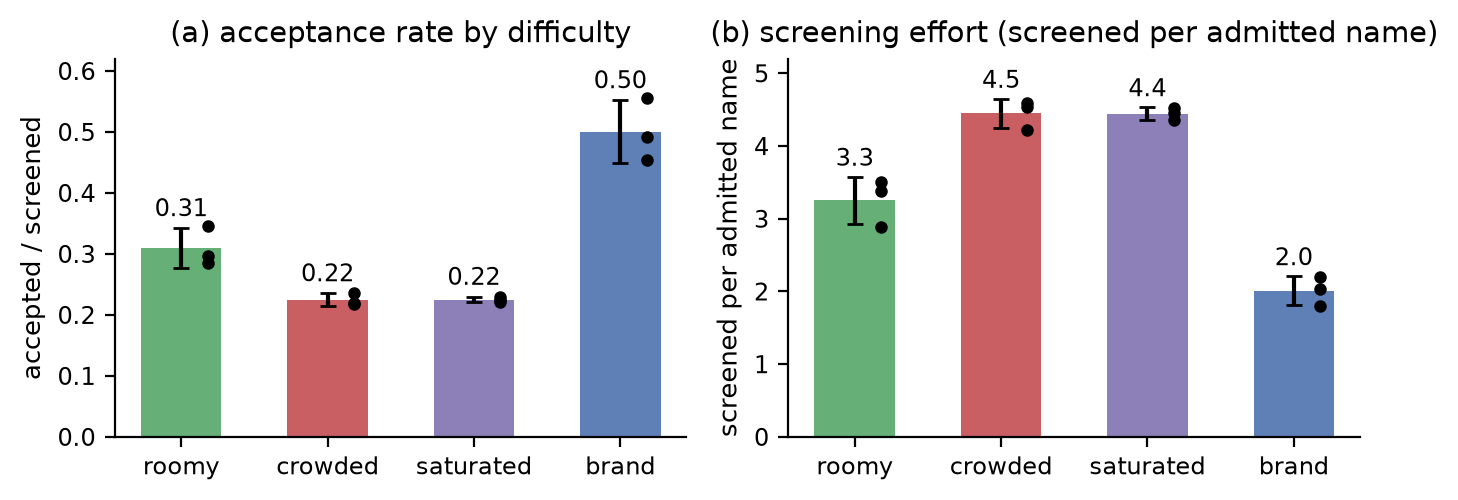
\includegraphics[width=\textwidth]{fig_strata.png}
\caption{Acceptance rate and screening effort by difficulty stratum across the
three seeds (bars: mean; whiskers: standard deviation; dots: per-seed values).
The seed spread is an order of magnitude larger for brand than for generic,
because brand shortlists are anchored by what the proposers draw in a given seed
while stem-governed ones are anchored by the mandated ending itself.}
\label{fig:strata}
\end{figure*}

\begin{table}[t]
\caption{Per-class sweep results merged over three seeds, shortlist size 10 in
all cases. The low/mod column counts risk bands over the admitted candidates.}
\label{tab:perclass}
\centering
\scriptsize
\setlength{\tabcolsep}{3.2pt}
\begin{tabular}{llrrrrr}
\toprule
Stem & Difficulty & Scr. & Adm. & Rate & Best $q$ & low/mod \\
\midrule
\code{-pril}      & roomy     &  196 & 100 & 0.510 & 71.27 & 5/95 \\
\code{-sartan}    & roomy     &  547 & 113 & 0.207 & 70.62 & 10/103 \\
\code{-vaptan}    & roomy     &  202 & 101 & 0.500 & 73.15 & 9/92 \\
\code{-dipine}    & roomy     &  411 & 103 & 0.251 & 72.83 & 4/99 \\
\code{-olol}      & crowded   &  194 & 114 & 0.588 & 71.69 & 13/101 \\
\code{-prazole}   & crowded   &  824 & 150 & 0.182 & 68.60 & 10/140 \\
\code{-caine}     & crowded   &  413 &  90 & 0.218 & 69.18 & 2/88 \\
\code{-statin}    & crowded   &  809 & 167 & 0.206 & 67.37 & 0/167 \\
\code{-cycline}   & crowded   &  732 & 148 & 0.202 & 68.18 & 16/132 \\
\code{-tinib}     & saturated &  623 & 124 & 0.199 & 71.45 & 2/122 \\
\code{-mab}       & saturated &  180 & 133 & 0.739 & 69.52 & 3/130 \\
\code{-gliptin}   & saturated &  814 & 119 & 0.146 & 66.51 & 21/98 \\
\code{-gliflozin} & saturated &  799 &  90 & 0.113 & 61.14 & 62/28 \\
\code{-parib}     & saturated &  185 & 119 & 0.643 & 72.45 & 6/113 \\
brand (all six)   & brand     & 1152 & 576 & 0.500 & 67.03 & 24/552 \\
\bottomrule
\end{tabular}
\end{table}

\subsection{Which checks do the rejecting?}

A check that never fires is either redundant or mis-thresholded, and either way
its presence in a methodology section is not supported by the data.
Table~\ref{tab:failures} gives the distribution of failure codes over the
5\,834 rejections; the shares exceed 1.0 in total because a candidate can fail
several checks at once.

\begin{table}[t]
\caption{Failure profile over 5\,834 rejected candidates (three seeds).}
\label{tab:failures}
\centering
\scriptsize
\begin{tabular}{lrr}
\toprule
Failure code & Count & Share \\
\midrule
\code{TRADEMARK\_HIT}                & 5324 & 0.913 \\
\code{INTRA\_STEM\_TOO\_CLOSE}       & 3314 & 0.568 \\
\code{SIMILARITY\_TOO\_HIGH}         & 1899 & 0.326 \\
\code{EXACT\_NAME\_COLLISION}        &   17 & 0.003 \\
\code{STEM\_MISUSE\_IN\_BRAND}       &    6 & 0.001 \\
\code{STEM\_FOREIGN\_EMBEDDED}       &    4 & 0.001 \\
\code{CROSSLINGUAL\_ADVERSE\_MEANING}&    1 & 0.000 \\
\bottomrule
\end{tabular}
\end{table}

Three checks account for essentially all rejections and the remaining four are
close to inert, which is not evidence that they are unnecessary. The
phonotactic check did not fire once across all three seeds, because the induced
grammar makes unpronounceable output structurally rare, so it is confirming that
the proposer works, and \code{STEM\_FOREIGN\_EMBEDDED} fires on names that would
otherwise have passed with a correct terminal stem and a contradictory internal
one. The trademark and intra-stem checks are the binding constraints; the others
are cheap insurance.

\subsection{Proposer contribution}

Both free proposers were run on every request, so their contributions can be
compared over logged pool data rather than by forcing a mode switch on the user
(Table~\ref{tab:proposer}).

\begin{table}[t]
\caption{Proposer contribution over the full three-seed sweep.}
\label{tab:proposer}
\centering
\footnotesize
\begin{tabular}{lrrrrr}
\toprule
Proposer & Prop. & Acc. rate & Mean $q$ & Best $q$ & Shortlist \\
\midrule
grammar            & 4251 & 0.266 & 63.60 & 75.33 & 0.692 \\
\code{ngram\_guided}& 3830 & 0.292 & 60.47 & 75.65 & 0.308 \\
\bottomrule
\end{tabular}
\end{table}

The two have near-identical acceptance rates, 0.266 against 0.292, and the
n-gram model produces the single highest-quality candidate of the sweep. Yet the
grammar proposer takes 69.2\% of shortlist slots, because acceptance and quality
are different questions and selection happens on the latter. This split is the
empirical case for pooling: a cascade running the n-gram model first and
stopping on its first admissible output would have been right about
admissibility and still produced a materially worse shortlist.

Refinement contributes disproportionately relative to its own acceptance rate.
Of 2\,296 refined attempts only 9.8\% were admitted, against 35.0\% for unrefined
candidates, but refined candidates carry a mean quality of 65.41 against 60.80
and occupy 137 of the 600 shortlist slots. Editing near-misses is a low-yield,
high-value operation, which is why it is restricted to the top 8 rejects.

\subsection{Does every quality term earn its place?}

Each term was removed in turn and the composite recomputed over the 6\,929
generic candidates in the sweep, and the result reported as a Spearman rank
correlation against the full objective, because what matters is whether removal
changes \emph{which names get picked}, not whether it shifts every score by a
constant (Table~\ref{tab:ablate-q}).

\begin{table}[t]
\caption{Quality-objective ablation, $n = 6\,929$ generic candidates (three
seeds).}
\label{tab:ablate-q}
\centering
\footnotesize
\begin{tabular}{lcccl}
\toprule
Term removed & $w$ & Rank corr. & $|\Delta q|$ & Reading \\
\midrule
novelty          & 0.20 & 0.545 & 5.06  & load-bearing \\
typicality       & 0.07 & 0.938 & 3.54  & contributes \\
pronounceability & 0.14 & 0.946 & 3.98  & contributes \\
shape            & 0.10 & 0.950 & 2.70  & contributes \\
morpheme hygiene & 0.16 & 0.991 & 6.79  & near-inert \\
seam             & 0.09 & 0.998 & 3.66  & near-inert \\
distinctiveness  & 0.24 & 0.999 & 19.58 & near-inert \\
\bottomrule
\end{tabular}
\end{table}

The result is uncomfortable and is reported as such. The
\emph{highest}-weighted term, distinctiveness at 0.24, shifts absolute scores by
19.58 points on average yet leaves the ranking almost untouched at a rank
correlation of 0.999. The reason is in the raw data: mean distinctiveness across
all screened generic candidates is 0.003 with a standard deviation of 0.021. The
term is saturated at zero, because it scores headroom below the 55 review line
and virtually every stem-conforming candidate lands above that line, so it
contributes a near-constant offset rather than a discriminating signal. Morpheme
hygiene is near-inert for the opposite reason, with a mean of 0.979 because the
induced grammar makes foreign morphemes structurally rare. Only novelty
genuinely reorders the shortlist, at 0.545.

%=============================================================================
\section{Discussion}

\subsection{The review band is a property of the problem}

Of the 600 names returned across the sweep, 528 (88.0\%) sit in the 55--70
review band and only 72 clear it outright. Rejecting the band outright was tried
and collapsed the admissible rate to roughly 0.5\%. The explanation is
structural rather than algorithmic: in a stem-governed class the mandated stem
is shared verbatim with every sibling, so a name complying with the regulation
is thereby forced into high orthographic similarity with the entire class.
Stem-aware scoring mitigates but does not eliminate this, because comparison
against the rest of the corpus still uses the full string.

The correct response is to report the band explicitly and let the quality
objective rank grey-band names below clear ones, which is why the objective
scores headroom against 55 rather than 70. Combined with
Table~\ref{tab:ablate-q}, however, the two facts compose awkwardly:
distinctiveness measured against 55 is exactly the term that saturates, so the
mechanism intended to demote grey-band names is the one with the least effect on
ranking. Rescaling it against the conditional score distribution within a class
is the obvious correction and is left to future work.

\subsection{What the audit trail looks like}

Table~\ref{tab:audit} contrasts a name the system returned with one its
predecessor returned, using the same screen; the converter transcribes
\code{lekurtolol} as \code{L EH K ER T OW L AO L}.

\begin{table}[t]
\caption{Audit trail for an admitted and a rejected candidate, \textnormal{\texttt{-olol}}.}
\label{tab:audit}
\centering
\scriptsize
\setlength{\tabcolsep}{3.5pt}
\begin{tabular}{lcc}
\toprule
 & \code{lekurtolol} & \code{erythroolol} \\
\midrule
Admissible               & yes           & \textbf{no} \\
Risk band                & moderate      & high \\
Composite risk $S$       & 60.21         & 76.15 \\
Nearest existing name    & \code{labetalol} & \code{erythrulose} \\
\quad orthographic / phonetic & 47.2 / 73.2 & 69.3 / 83.0 \\
Margin to review (55)    & $-5.21$       & $-21.15$ \\
Margin to reject (70)    & $+9.79$       & $-6.15$ \\
Syllables                & 4             & 5 \\
Phonotactic / typicality & 1.00 / 0.011  & 1.00 / 0.176 \\
\midrule
Quality total            & \textbf{68.98} & \textbf{27.24} \\
\quad novelty            & 1.000         & 0.150 \\
\quad morpheme hygiene   & 1.000         & 0.120 \\
\quad seam               & 1.000         & 0.350 \\
\quad shape              & 0.998         & 0.821 \\
\bottomrule
\end{tabular}
\end{table}

\code{erythroolol} is rejected on similarity to \code{erythrulose} at 76.15 and
independently scores 0.150 on novelty and 0.120 on morpheme hygiene because
\code{erythro} is a real class-signalling morpheme: two signals pointing at the
same defect from different directions, which is the intended redundancy.

%=============================================================================
\section{Limitations}

\textbf{This is a first-pass screen.} It contains no prescription-simulation
human-factors study, no legal likelihood-of-confusion analysis and no committee
judgement, all part of an actual regulatory review
\cite{fdaguidance,emaguideline}. A low band means \emph{worth taking to
review}, never \emph{cleared}.

\textbf{The universe bounds the claim.} Distinctiveness is measured against the
assembled corpus of 19\,635 names, so every reported margin is an upper bound.
The EMA feed failed to retrieve in the runs recorded here, leaving European-only
products represented solely through the committed snapshot.

\textbf{Phonetics are orthographic and Anglocentric.} The grapheme-to-phoneme
converter is rule-based and English-oriented, and the cross-lingual check is a
68-term lexicon lookup, not a phonological model of each market language.

\textbf{The trademark check is a proxy.} It screens against marketed proprietary
names, not against a registered trademark class search, which is a legal
instrument and not reproducible from open data.

\textbf{The validation set is small.} Thirty documented confusable pairs is a
strong label but a thin sample, and the component ablation in
Table~\ref{tab:ablate-sim} is underpowered as a result: a difference of 0.0005 in
AUC over 30 positives is not a meaningful effect size.

\textbf{Residual artefacts survive selection.} The \code{-olol} shortlist
includes \code{ipqolol}, whose \code{pq} sequence passes the phonotactic check on
the transcribed phoneme string but reads poorly: the check tests syllable-level
legality and does not penalise low-frequency orthographic sequences directly.

%=============================================================================
\section{Conclusion and Future Work}

This paper describes a generative--verifier architecture that treats
pharmaceutical naming as a constrained search problem in which generation and
regulatory screening form one closed loop rather than two disconnected tools.
The screen discriminates documented confusable pairs from random corpus pairs at
a ROC AUC of 0.997 with a mean separation of 39.9 points, and the generator
returns a full shortlist for all twenty targets of a difficulty-stratified sweep
at three seeds, admitting 27.8\% of 8\,081 screened candidates entirely on CPU
with no API dependency. The two pipelines deliver the opposed behaviours their
regulatory mandates demand: generic targets accept at $0.241$ while brand
targets accept at $0.501$, and the best generic shortlist quality exceeds the
best brand one.

Four results point at future work. The moderate-similarity band absorbs 88\% of
returned names because a mandated stem forces similarity to siblings, so the
distinctiveness term should be rescaled against the conditional score
distribution within a class rather than a fixed line. The similarity-component
ablation is underpowered at 30 labelled pairs; extending the ground truth to the
full published ISMP list with severity weighting would test the phonetic
component properly. The near-inert highest-weighted term is a standing
invitation to re-derive the objective's weights from data rather than by hand.
Finally, replacing the Anglocentric rule-based converter with a multilingual
grapheme-to-phoneme model would turn the cross-lingual check into a phonological
screen rather than a lexicon lookup.

%=============================================================================
\begin{thebibliography}{00}

\bibitem{lambert1999}
B.~L. Lambert, S.-J. Lin, K.-Y. Chang, and S.~K. Gandhi, ``Similarity as a risk
factor in drug-name confusion errors,'' \emph{Med. Care}, vol.~37, no.~12,
pp.~1214--1225, Dec. 1999, doi: 10.1097/00005650-199912000-00005.

\bibitem{ismp}
Institute for Safe Medication Practices, ``ISMP list of confused drug names,''
ECRI/ISMP, Plymouth Meeting, PA, USA, 2023.

\bibitem{fdapoca}
U.S. Food and Drug Administration, ``Phonetic and Orthographic Computer Analysis
(POCA) program,'' Silver Spring, MD, USA, 2023. [Online]. Available:
\url{https://www.fda.gov/drugs/resources-drugs}

\bibitem{fdaguidance}
U.S. Food and Drug Administration, ``Best practices in developing proprietary
names for human prescription drug products: Guidance for industry,'' CDER,
Silver Spring, MD, USA, Dec. 2020.

\bibitem{emaguideline}
European Medicines Agency, ``Guideline on the acceptability of names for human
medicinal products processed through the centralised procedure,'' rev.~7,
Amsterdam, Netherlands, 2023.

\bibitem{whostem}
World Health Organization, \emph{The Use of Stems in the Selection of INN for
Pharmaceutical Substances}. Geneva, Switzerland: WHO, 2018,
WHO/EMP/RHT/TSN/2018.1.

\bibitem{usanstems}
American Medical Association, ``United States Adopted Names approved stems,''
Chicago, IL, USA, 2024. [Online]. Available:
\url{https://www.ama-assn.org/about/united-states-adopted-names-usan}

\bibitem{kondrak2006}
G.~Kondrak and B.~Dorr, ``Automatic identification of confusable drug names,''
\emph{Artif. Intell. Med.}, vol.~36, no.~1, pp.~29--42, Jan.
2006, doi: 10.1016/j.artmed.2005.07.005.

\bibitem{kondrak2004}
G.~Kondrak and B.~Dorr, ``Identification of confusable drug names,'' in
\emph{Proc. 20th Int. Conf. Computational Linguistics (COLING '04)}, Geneva,
Switzerland, 2004, art. no.~952, doi: 10.3115/1220355.1220492.

\bibitem{levenshtein1966}
V.~I. Levenshtein, ``Binary codes capable of correcting deletions, insertions,
and reversals,'' \emph{Sov. Phys. Dokl.}, vol.~10, no.~8, pp.~707--710,
Feb. 1966.

\bibitem{kondrak2000}
G.~Kondrak, ``A new algorithm for the alignment of phonetic sequences,'' in
\emph{Proc. 1st Meeting North American Chapter Assoc. Computational
Linguistics (NAACL)}, Seattle, WA, USA, 2000.

\bibitem{zobel1996}
J.~Zobel and P.~Dart, ``Phonetic string matching: Lessons from information
retrieval,'' in \emph{Proc. 19th Annu. Int. ACM SIGIR Conf.}, Zurich, Switzerland, 1996,
pp.~166--172, doi: 10.1145/243199.243258.

\bibitem{emmerton2020}
L.~Emmerton, C.~Curtain, G.~Swaminathan, and H.~Dowling, ``Development and
exploratory analysis of software to detect look-alike, sound-alike medicine
names,'' \emph{Int. J. Med. Informat.}, vol.~137, art. no.~104119, May 2020, doi: 10.1016/j.ijmedinf.2020.104119.

\bibitem{lambert2015}
B.~L. Lambert, R.~Bhaumik, W.~Zhao, and D.~K. Bhaumik, ``Detection and
prediction limits for identifying highly confusable drug names from experimental
data,'' \emph{J. Biopharm. Statist.}, vol.~26, no.~2, pp.~365--385, 2016, doi: 10.1080/10543406.2015.1052481.

\bibitem{geng2023}
S.~Geng, M.~Josifoski, M.~Peyrard, and R.~West, ``Grammar-constrained decoding
for structured NLP tasks without finetuning,'' in \emph{Proc. 2023 Conf.
Empirical Methods in Natural Language Processing (EMNLP)}, Singapore, Dec. 2023,
pp.~10932--10952, doi: 10.18653/v1/2023.emnlp-main.674.

\bibitem{holtzman2020}
A.~Holtzman, J.~Buys, L.~Du, M.~Forbes, and Y.~Choi, ``The curious case of
neural text degeneration,'' in \emph{Proc. Int. Conf. Learning Representations
(ICLR)}, Addis Ababa, Ethiopia, 2020.

\bibitem{liu2024}
X.-h. Liu, Z.-h. Lu, T.~Wang, and F.~Liu, ``Large language models facilitating
modern molecular biology and novel drug development,'' \emph{Front. Pharmacol.}, vol.~15, art. no.~1458739, 2024, doi: 10.3389/fphar.2024.1458739.

\bibitem{rxnorm}
S.~J. Nelson, K.~Zeng, J.~Kilbourne, T.~Powell, and R.~Moore, ``Normalized names
for clinical drugs: RxNorm at 6 years,'' \emph{J. Amer. Med. Informat. Assoc.}, vol.~18, no.~4, pp.~441--448, Jul. 2011,
doi: 10.1136/amiajnl-2011-000116.

\bibitem{openfda}
T.~A. Kass-Hout \emph{et al.}, ``OpenFDA: An innovative platform providing
access to a wealth of FDA's publicly available data,'' \emph{J. Amer. Med. Informat. Assoc.}, vol.~23, no.~3, pp.~596--600, May 2016,
doi: 10.1093/jamia/ocv153.

\end{thebibliography}

\end{document}